\documentclass[hidelinks,a4paper,11pt]{article}
\usepackage[margin=2cm]{geometry}

\usepackage[titletoc,toc,title,page]{appendix}
\usepackage[nodayofweek]{datetime}
\usepackage{cite}
\usepackage{graphicx}
\longdate

\usepackage{hyperref}
\usepackage{fancyhdr}
\pagestyle{fancyplain}


\begin{document}


\section{Target animation}

For the sake of testing, we needed a video input, that would represent dragonfly's vision. We started with suggestion of creating 3D animation that would be exactly as dragonfly's vision, 180 degree sphere. Creating such an animation would pose quite a challenge and would be an overkill for our needs. We boiled down out needs to two things: a sort of moving target and a moving background. We could represent this with 2D animation of circles moving through the screen and a background picture, which would be moving as well. Our priorities were flexibility and simplicity. Erik was assigned a task of creating a module, which would satisfy above needs.

Erik started design looking from the user's perspective. User would want to add targets, a background and get a final product. This could be done with 3 functions that would interact with an interface class. We named that class Animation. There were two types of targets: randomly moving ones and straight line moving ones. For randomly moving ones, one could set a starting position and speed. In addition one should set vector of movement for targets moving in straight line. Background is represented with directory of picture and a speed with which we want it to move. Target and Background are both encapsulated in a class.

Next challenge was, how to turn this information into an animation. Decision was made to first create a sequence of images and turn them into an animation at the very end. Christos suggested a Python's library Gizzet for image creation. It offers exactly what we needed – drawing circles, adding pictures etc. We use user's input to calculate position of each target and of background at each frame. Using that calculation we know where to draw circles and background picture, afterwards we save created image.

Generated sequence of images is than combined using library OpenCV. There exists a parameter setting format of video output. Video is created and exported under selected name. This final product is then imported in ESTMD module to isolate targets.

In addition to the above functionality of target animation module, we needed to somehow pass data of target positions to the final module – action selection – in order to estimate its efficiency. To satisfy this need we added functions that calculate positions of targets at certain time. As an argument we didn't use frame, but we used time in interval [0, 1]. We decided for this to avoid any synchronization problems that might arise over all the modules.

For final presentation, user can also add dragonfly's path. Dragonfly is represented with large red circle.
Example of frame in produced video can be seen on the picture  ~\ref{target_animation_example}.

\begin{figure}[hb]
\centering
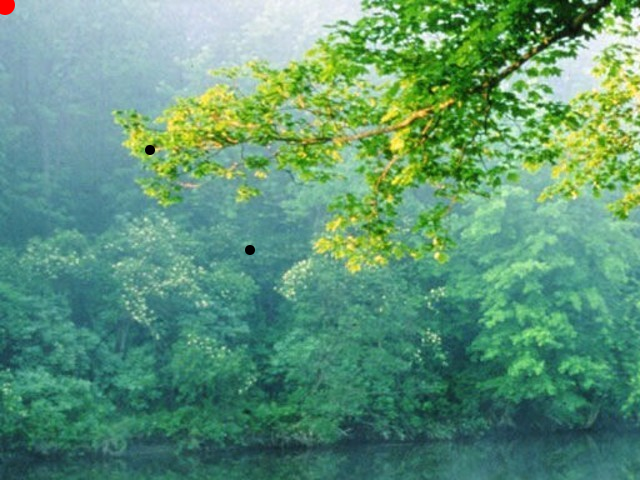
\includegraphics[scale = 0.3]{example}
\caption{Simple example of action selection output. The red dot represents the dragonfly focal point and the black dot represents the target.}
\label{target_animation_example}
\end{figure}



\end{document}

